%----------------------------------------------------------------------------------------
%	PACKAGES AND OTHER DOCUMENT CONFIGURATIONS
%----------------------------------------------------------------------------------------

\documentclass[paper=a4, fontsize=11pt]{scrartcl} % A4 paper and 11pt font size

\usepackage[T1]{fontenc} % Use 8-bit encoding that has 256 glyphs
\usepackage{fourier} % Use the Adobe Utopia font for the document - comment this line to return to the LaTeX default
\usepackage[english]{babel} % English language/hyphenation
\usepackage{amsmath,amsfonts,amsthm} % Math packages

\makeatletter
%\renewcommand\thesection{}
%\renewcommand\thesubsection{\@arabic\c@section.\@arabic\c@subsection}
\makeatother

\usepackage{fancyhdr} % Custom headers and footers
\pagestyle{fancyplain} % Makes all pages in the document conform to the custom headers and footers
\fancyhead{} % No page header - if you want one, create it in the same way as the footers below
\fancyfoot[L]{} % Empty left footer
\fancyfoot[C]{} % Empty center footer
\fancyfoot[R]{\thepage} % Page numbering for right footer
\renewcommand{\headrulewidth}{0pt} % Remove header underlines
\renewcommand{\footrulewidth}{0pt} % Remove footer underlines
\setlength{\headheight}{13.6pt} % Customize the height of the header

%\numberwithin{equation}{section} % Number equations within sections (i.e. 1.1, 1.2, 2.1, 2.2 instead of 1, 2, 3, 4)
%\numberwithin{figure}{section} % Number figures within sections (i.e. 1.1, 1.2, 2.1, 2.2 instead of 1, 2, 3, 4)
%\numberwithin{table}{section} % Number tables within sections (i.e. 1.1, 1.2, 2.1, 2.2 instead of 1, 2, 3, 4)

%\setlength\parindent{0pt} % Removes all indentation from paragraphs - comment this line for an assignment with lots of text

\usepackage{graphicx}
\usepackage{caption}
\usepackage{subcaption}
\usepackage{algorithm2e}
\usepackage{booktabs}

\newcommand{\code}[1]{{\footnotesize\textsf{#1}}}
\newcommand{\q}[1]{``#1''}

\usepackage{listings}

\usepackage{geometry}
\geometry{letterpaper, margin=1.95cm}

\usepackage{url}

%\usepackage{multirow}


%----------------------------------------------------------------------------------------
%	TITLE SECTION
%----------------------------------------------------------------------------------------

\newcommand{\horrule}[1]{\rule{\linewidth}{#1}} % Create horizontal rule command with 1 argument of height

\title{	
\normalfont \normalsize 
\textsc{Utah State University, Computer Science Department} \\ [25pt] % Your university, school and/or department name(s)
\horrule{0.5pt} \\[0.4cm] % Thin top horizontal rule
\huge CS5890 Data Science - Project Proposal \\ Random Acts Of Pizza \\ % The assignment title
\horrule{2pt} \\[0.5cm] % Thick bottom horizontal rule
}

\author{Team \textbf{Pizza Hackers}: Tam Nguyen and Hung Pham} % Your name

\date{\normalsize\today} % Today's date or a custom date

\begin{document}
	
\maketitle
	
\section{Introduction}

In this proposal we will discuss our plan to perform data analysis on a social interaction dataset, where requester ask for free pizza on a Reddit community \q{Random Acts of Pizza}\footnote{\url{https://www.reddit.com/r/Random_Acts_Of_Pizza/}}. We will discuss the social interaction problems, the dataset provided by Kaggle, preliminary of our analysis plan, which data science toolkits we plan to use.

\section{The team: Pizza hackers}

We name our team \q{Pizza hackers} in direct references to the task that we want to tackle, and our Computer Scientist's root. \q{Pizza hackers} consists of two members: Tam Nguyen and Hung Pham. Tasks such as implementations of data analysis experiments, report writing, and visualization will be divided among team members. All members will be involved in analysis of experiments results as well as any decision in term of project direction.

\section{The problems}

Internet is a newly discover virtual land, where humans interact with each others on multiple levels. Interaction with a new person on-line is only a few mouse clicks away. It is an active researching field to study the interaction between humans in a virtual space. Study how human response to request from a complete stranger is an interesting research question. Crown-funding has been one of the best way for startup companies and inventors to acquire necessary funding.\\

Althoff \emph{et al} have investigate which factors effect the successfulness of a request \cite{tim14}, specifically requests for free pizzas. They used topic modeling and logistic regression to determine which narrative topic have the highest success rate and in turn determine factors that effect the outcome of a request such as: who is asking, how the request was asked. We decided to extend this research by using a different set of techniques that are more up-to-date such as distributed vector representation (Word2Vec\cite{word2vec}) and Support Vector Machine. We will discuss the details of our plan in The plan section.\\



\section{The dataset}
We downloaded data from Kaggle\footnote{\url{https://www.kaggle.com/c/random-acts-of-pizza/download/train.json.zip}}. The dataset includes 4040 requests collected from the Reddit community Random Acts of Pizza between December 8, 2010 and September 29, 2013. Each data object is a request for a free pizza. There are 994 requests received a pizza while 3046 requests did not. \\

The dataset is in \texttt{JSON} format. Each \texttt{JSON} entry represents one pizza request. Data fields includes information about requests such as id, text, requester name, etc. and meta-data such as: time of the request, activity of the requester, community-age of the requester, etc. There are several fields are collected after the time a request was posted, the values of those fields doesn't affect whether a request receive pizza, thus, we removed those fields out of the dataset. Table \ref{fields} shows important attributes (and explanations that) we consider in our analysis.

\begin{table}[]
	\sf\scriptsize
	\centering
	\caption{Important attributes used in our analysis}
	\label{fields}
	\begin{tabular}{lp{10cm}}
		\toprule
		Important Attributes                              & Explanations                                                                          \\
		\midrule
		\multicolumn{2}{l}{Request text}                                                                                                        \\
		\midrule
		request\_title                                    & Title of the request                                                                  \\
		request\_text\_edit\_aware                        & Request text after removing comments indicating the success of the request            \\
		\midrule
		\multicolumn{2}{l}{Requester information}                                                                                                 \\
		\midrule
		requester\_account\_age\_in\_days\_at\_request    & The age of requester (in days) at time of request                                     \\
		requester\_number\_of\_comments\_at\_request      & The number of comments on Reddit by requester at time of request                      \\
		requester\_number\_of\_posts\_at\_request         & The number of posts on Reddit by requester at time of request.                        \\
		requester\_subreddits\_at\_request                & The number of subreddits that requester had posted in at the time of request. \\
		requester\_upvotes\_minus\_downvotes\_at\_request & Difference of upvotes and downvotes of requester at time of retrieval.                \\
		requester\_upvotes\_plus\_downvotes\_at\_request  & Sum of  upvotes and downvotes of requester at time of request.                        \\
		\bottomrule
	\end{tabular}
\end{table}

\section{The plan}

\begin{figure}
	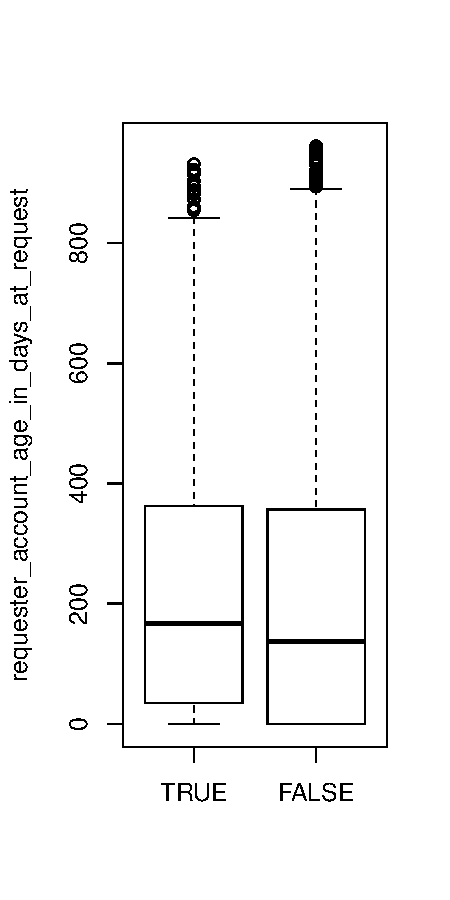
\includegraphics[width=0.19\textwidth]{data/requester_account_age_in_days_at_request}
	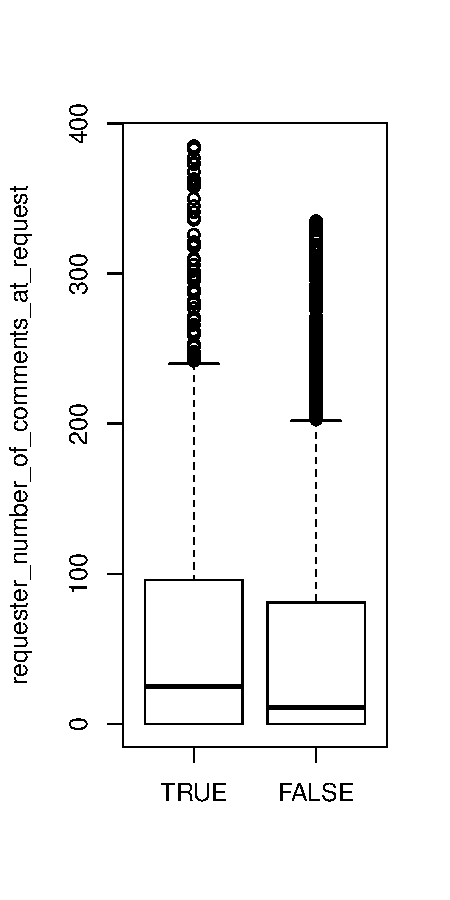
\includegraphics[width=0.19\textwidth]{data/requester_number_of_comments_at_request}
	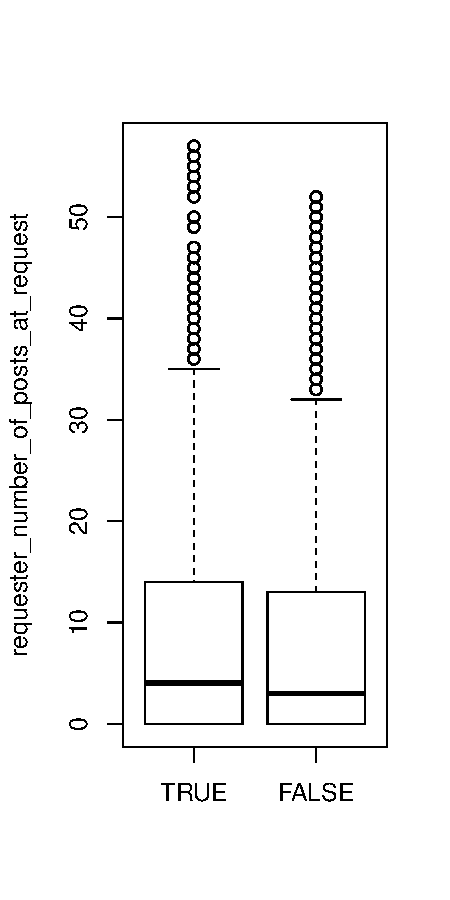
\includegraphics[width=0.19\textwidth]{data/requester_number_of_posts_at_request}
	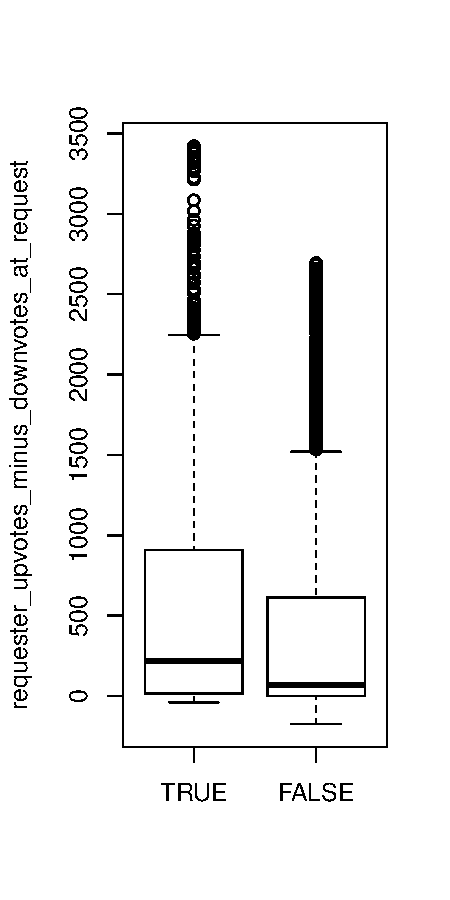
\includegraphics[width=0.19\textwidth]{data/requester_upvotes_minus_downvotes_at_request}
	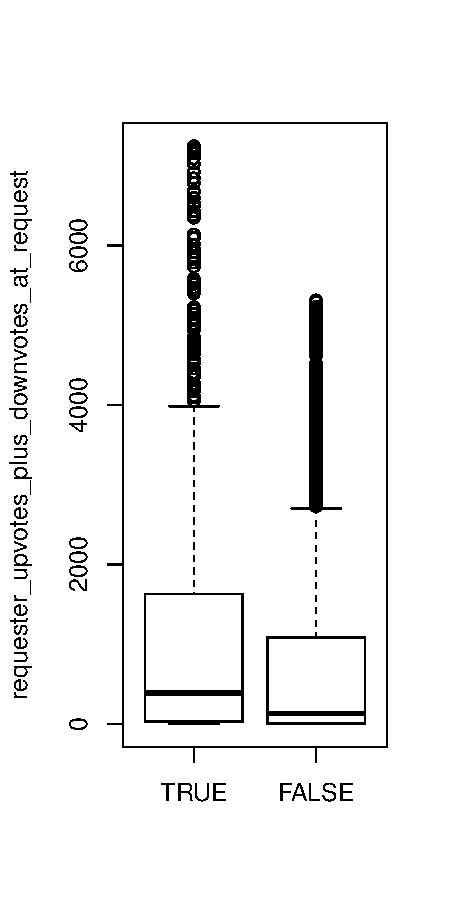
\includegraphics[width=0.19\textwidth]{data/requester_upvotes_plus_downvotes_at_request}
	\caption{Boxplots of some attributes based on the success of requests}
	\label{boxplot}
\end{figure}

To analyze our data we will perform three critical steps:

\begin{itemize}
	\item General analysis of simple information about requesters.
	\item General analysis of textual attributes (request subject and body).
	\item Apply prediction model to measure effectiveness of each factor.
\end{itemize}

For example, we could perform comparison between successful and unsuccessful requests to see if an older account holder will have more chance at receiving a free pizza or not using a simple box plot of the attribute \textit{requester\_account\_age\_in\_days\_at\_request}. Table~\ref{boxplot} is showing such analysis for the five most interesting attributes containing requester information. We will also apply prediction model such as logistic regression using different attribute to see which one have the best predictive power. Such analysis will give us some idea of how the information available in Reddit about the requesters could effect the outcome.\\

The two most interesting and valuable attributes in our dataset are \textit{request\_title} and \textit{request\_text\_edit\_aware}. These attributes contain the title and textual body of each request. Most of decision will be based upon the contents of these two attributes. We will first performing some preprocessing including:  tokenizing, stop-word removal, stemming... Then we will use a simple frequency based phrase builder to create phrases that occurred enough but not too much or too little (The details will be included in check point report). We could then investigate the relationship between terms and phrases that co-occur the most with successful and unsuccessful requests. We could also use simple logic regression to see which terms or phrases have the most predictive power.\\

Finally, we will apply Word2Vec on these textual attributes to extract vector representation of terms and phrases, then by using clustering we could be able to find cluster of terms and phrases that have similar syntactic and semantic meaning. We then extract the \q{bag-of-cluster} vector for each request and feed this to SVN so that the model can learn to predict the outcome. By investigate the weight vector of SVN model we will be able to tell which cluster (factor) have the most effect on the outcome.




\section{The Toolkits}
We plan to use \texttt{R} as the main programming language in our analysis. We have used \texttt{jsonlite} library for importing dataset (in \texttt{JSON} format) to dataframe in \texttt{R}. We also used \texttt{R} to produce boxplots in our preliminary analysis. All attributes about requester are quantitative, thus, using \texttt{R} as the analysis language is sufficient. For analyzing textual data, we plan to use \texttt{word2vec} library\footnote{\url{https://code.google.com/p/word2vec/}}. For building classifier to predict whether a request receive a pizza we plan to use \texttt{R} interface of \texttt{libsvm}\footnote{\url{https://www.csie.ntu.edu.tw/~cjlin/libsvm/}} library.

\begin{thebibliography}{10}

\bibitem{tim14}
Tim Althoff, Cristian Danescu-Niculescu-Mizil, Dan Jurafsky.
\emph{How to Ask for a Favor: A Case Study on the Success of Altruistic Requests},
Proceedings of ICWSM,
2014.

\bibitem{word2vec}
Tomas Mikolov, Ilya Sutskever, Kai Chen, Greg S Corrado, Jeff Dean.
\emph{Distributed representations of words and phrases and their compositionality},
Advances in neural information processing systems,
2013.


\end{thebibliography}

\end{document}